\documentclass{article}
\setlength{\columnsep}{20pt}
%\usepackage{url}
%\usepackage{algorithmic}
\usepackage[a4paper]{geometry}
\usepackage{datetime}
\usepackage[font=small,labelfont=it]{caption}
\usepackage{mathpazo} % use palatino
\usepackage[scaled]{helvet} % helvetica
\usepackage{microtype}
\usepackage{amsmath}
\usepackage{subfigure}
\usepackage{hyperref}
\usepackage[export]{adjustbox}
\usepackage{multicol}% http://ctan.org/pkg/multicols
\usepackage{float}
\usepackage{graphicx}
 
% Letterspacing macros
\newcommand{\spacecaps}[1]{\textls[200]{\MakeUppercase{#1}}}
\newcommand{\spacesc}[1]{\textls[50]{\textsc{\MakeLowercase{#1}}}}

\usepackage[utf8]{inputenc}
\usepackage{textgreek}
\usepackage[LGR,T1]{fontenc}
\usepackage{palatino}

\title{\vspace{-2.0cm}\spacecaps{WarInspector: Visual Analytics web application on Arms Transfer}\\ \normalsize \spacesc{Visual Analytics Course - Sapienza University of Rome} }

\author{Giuseppe Capaldi 1699498\\ Gianmarco Cariggi 1698481}
%\date{\today\\\currenttime}%
\date{\today}



\begin{document}
\maketitle
\begin{abstract}

In this report we present you "WarInspector", a web application embedding D3.js framework to visualize and let analyze data regarding world weapons trading. The web pages contain user interactive visualizations all coordinated on user actions. Among the views we have bar plots, cloropleth maps, scatter plot with PCA (Principal Component Analysis) data, computed on the back-end server and visualized not to preprocess the original dataset but to add new information to the user. The app is composed of two interconnected pages using the same datasets but focusing on the two main study cases we identified:  analysis on geopolitical and military influences between countries on one side and analysis of weapon's models in use. A demo of the application can be found at:
\url{https://war-inspector.herokuapp.com/}. The code is available at: \url{https://github.com/GiuppoUni/warInspector/}
%
\end{abstract}




\begin{multicols}{2}

\section*{Introduction}
%
The war has characterized the human being since the prehistory. Human beings have always tried to impose their strength and knowledge on other animals but also on their fellow humans. However, only a few centuries ago war has also become a business, where national war industries or more generally countries can do business and get rich without the effective use of military force. Our project aims to explore this theme, offering the user a visual analysis tool to better understand the dynamics behind this increasingly profitable market.

We developed a web application that is designed for all possible war or investigative operators or journalists who want to understand how this market moves, in particular by analysing the trading of arms between countries and how conflicts can be geographically or diplomatically related/unrelated. The tool makes it possible to understand from a quantitative point of view, evaluating the numbers of units traded (imported or exported) and also how these numbers can be somehow influenced by other parameters characterizing the country (population, GDP, army dimensions), which at first glance may seem detached from this area. From a qualitative point of view, on the other hand, the application analyses categories and specific models of weapons that are exchanged, along with the possibility to explore details of a single transaction. This allows a hypothetical arms producer to understand which weapons are the most traded in a certain historical period or in a particular region and the presence of past economic trends to exploit. 
For both cases the single transactions can be finely filtered to explore interesting or suspicious ones.

The paper is organized as follows: in the first section we are going to explain the content of our datasets, the sources and how we have combined them together; in the second section we will discuss the study cases from which we designed the app; in the third section instead we will focus on the design choices we took; then in the fourth and fifth sections we will focus on the details of views; finally we will conclude with a discussion on the results and some food for thought.

\section{Use cases}
The first study case we thought of was the one of an investigation regarding geopolitical relations among countries. Weapons transactions from one country to another in a particular year or in some range of years could reveal  known or hidden alliances, or the attempts to circumvent restrictions imposed on the arms trading toward particular countries (weapons can be sold to countries bordering to banned countries to then carry secretly by land). Moreover the presence of consistent weapon transactions in an area related to past conflicts may reveal the risk of a future new conflict. For this purpose a banner in the upper right corner can be displayed on button press to see countries currently considered at risk of conflict based on external sources.

The second study case is more focused on the economic nature of the transactions, a market survey can be conducted integrating the first page of WarInspector with the second one, in which weapons are grouped by category and then on select by model to see which were the most traded weapons in certain situations. 



\section{Dataset and sources}
%


In order to offer a data visualization work that would have been interesting in his results, we chose to think of a dataset that could involve the entire planet and containing  information of social interest. Searching on the web the SIPRI website stood out cause of the possibility it offers to analyse and visualise datasets regarding military trade (from official reports of NATO and every single country which participates to this initiative) among countries. The dataset contains these information: suppliers and recipients, the type and number of weapon systems ordered and delivered, the years of deliveries and the financial value of the deal (but only for a few entries). 

To have a dataset ready to be easily visualized we needed a well formatted file, a \textit{CSV} (Comma Separated Values) would have been ideal, but the only format offered for our specific dataset of interest (the army transfer database) was \textit{RTF} (Rich Text Format), that is better to visualize a text due to the presence of text formatting elements, less for storing and visualize a dataset. So we downloaded from: \url{http://armstrade.sipri.org/armstrade/page/trade_register.php} selecting all suppliers, all recipients from 1990 to 2018 (2019 was not present at the time), all weapon systems and clicking onto "from supplier register". So after a quick analysis of its content, some Python scripts helped us to reach our CSV file containing a dataset with this format [Table 1]:
\begin{itemize}
\item \textbf{Ordered}: the number of items ordered under the deal;
\item \textbf{Weapon model}: the designation of the weapon system concerned;
\item \textbf{Weapon category}: description of the weapon system concerned;
\item \textbf{Ordered year}: the year the order was placed or, in the case of licensed production, the licence was issued;
\item \textbf{Delivered year}: the year or years during which deliveries took place. If none have yet been made, this field is left blank;
\item \textbf{Delivered num}: the number of items delivered or produced under the deal;
\item \textbf{Comments}: any additional information that is known about the deal. This can include the financial value of the deal, what the weapons will ostensibly be used for, whether they are being donated as military aid, and any information on offsets linked to the deal.
 
\end{itemize}
%%% Big Tables

\begin{center}
	\begin{table*}[hbt!]
		\resizebox{\textwidth}{!}{
			\begin{tabular}{||c|c|c|c|c|c|c|c|c||}
				\hline
				Supplier & Recipient & Ordered & Weapon model & Weapon category & Ordered year & Delivered year & Delivered num. & Comments             \\
				\hline
				...         &              &         &              &                 &              &                &                &                      \\
				\hline
				Albania  & Burkina Faso & (12)    & M-43 120mm   & Mortar          & (2011)       & 2011           & 12             & Probably second-hand \\
				\hline
				...         &              &         &              &                 &              &                &                &             \\ 
				\hline       
		\end{tabular}}
		
		\label{tab: d1}
		\caption { \label { tab:d1} Attributes of dataset in \texttt{Trade-Register-1990-2018.csv} file.  }
		
	\end{table*}
\end{center}




\begin{center}
	\begin{table*}[hbt!]
		\resizebox{\textwidth}{!}{
			\begin{tabular}{||l|l|l|l|l|l|l|l|l|l|l|l|l|l|l|l|l|l|l|l|l||}
				
				
				\hline
				& 1989 & ... & 2002 & 2003 & 2004 & 2005 & 2006 & 2007 & 2008 & 2009 & 2010 & 2011 & 2012 & 2013 & 2014 & 2015 & 2016 & 2017 & 2018 & 2019 \\
				\hline
				...       &      &      &      &      &      &      &      &      &      &      &      &      &      &      &      &      &      &      &      &      \\
				\hline
				Australia &    13  & ...   & 47   & 44   & 2    & 49   & 14   & 18   & 26   & 80   & 115  & 143  & 45   & 54   & 97   & 87   & 134  & 98   & 38   & 148  \\
				\hline
				...       &      &      &      &      &      &      &      &      &      &      &      &      &      &      &      &      &      &      &      &     \\
				\hline
				
			\end{tabular}[hbt!]
		}
		\label{tab:d2}
		
		\caption { \label { tab:d2} Attributes of dataset in \texttt{importNumbers1989-2018.csv} file.   }
		
	\end{table*}
	
\end{center}

In a second phase in order to better interact with the map we joined the said dataset with a second one containing only latitude-longitude coordinates and country code for both \textit{Supplier} and \textit{Recipient}. This new attributes have been used exclusively for visualization purposes.

To increase the dimensionality of our dataset, to be later computed using \textit{PCA}, we introduced other information for each country and for each year adding parameters as \textit{GDP}, \textit{population}, \textit{army dimensions}, \textit{number of escaped refugees} taken from open data website: \url{https://data.worldbank.org/}. 
Together with these features we have the import or export numbers (depending on user choice) that are taken from two different \textit{SIPRI} datasets [Table 2]. This is because they contain a trend-indicator value \textit{TIV}, to have for each year an exact number representing efficiently how many weapons a country exported/imported. This value takes into account several factors for a consistent measure to compare trades, different for number of units, type of weapon ecc.
Finally we added a removable bubble plot overlay on maps to display conflicts happened in a certain region, this data has been obtained from the website: \url{http://www.systemicpeace.org/warlist/warlist.htm} along with an alert banner containing countries with high risk of a new conflict, taken from:  \url{https://www.crisisgroup.org/crisiswatch}.  





Next you can find a figure displaying the involved datasets and the process of merging:

\begin{figure}[H]

		\centering
	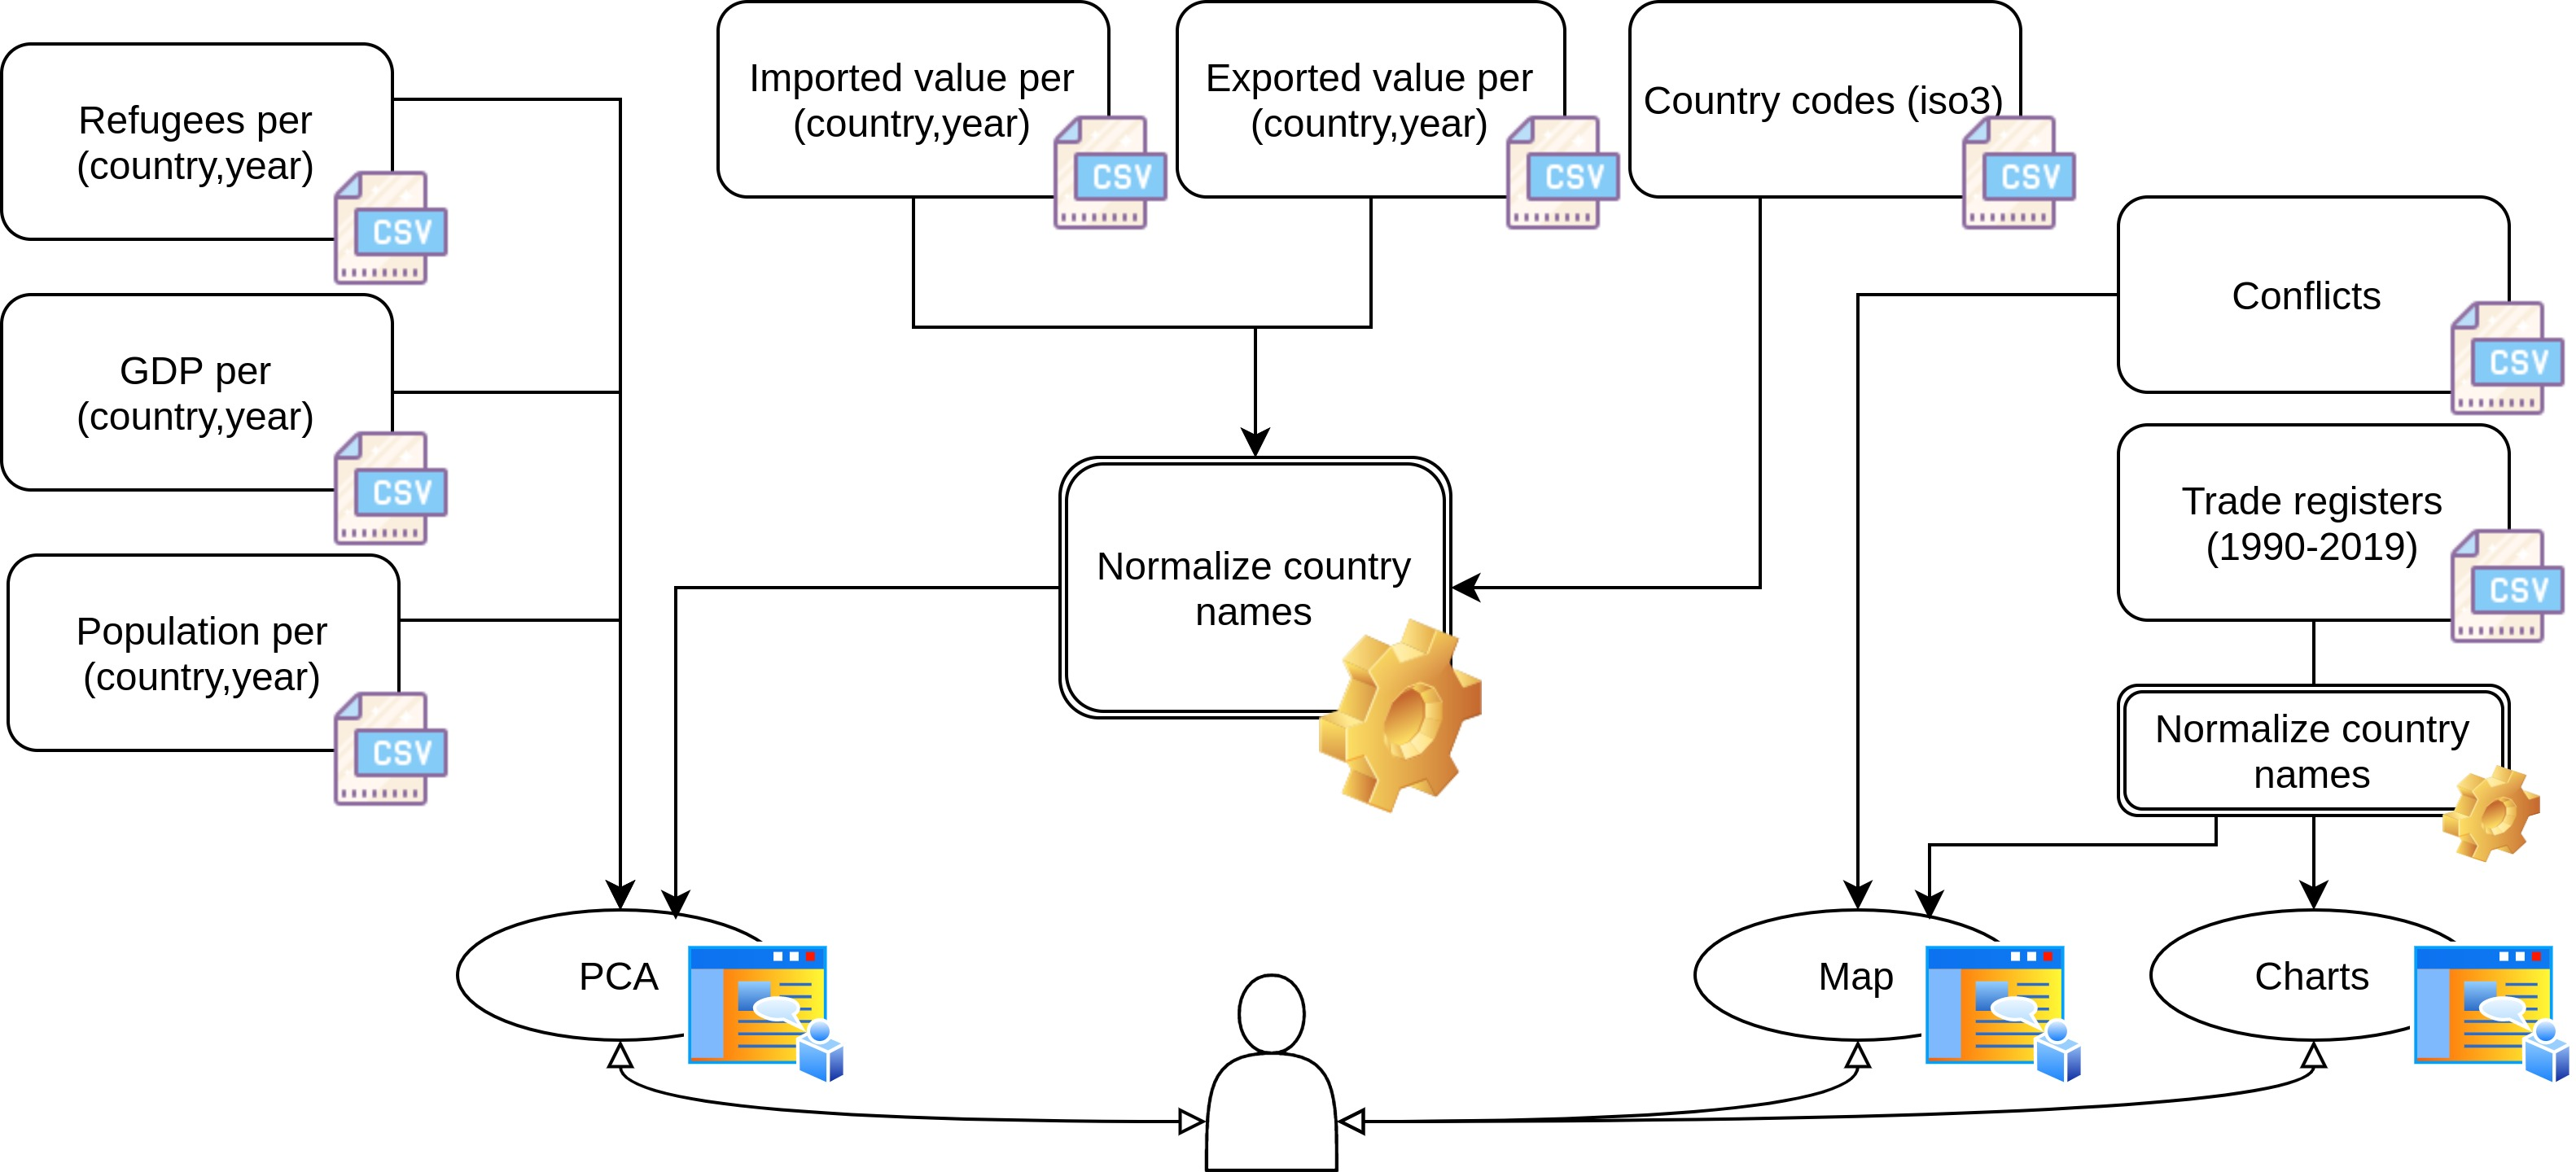
\includegraphics[scale=0.07,center]{./fig/vaBigDataIcons2.jpg}
	\label{fig:vaBigData}
	\caption{Summering schema to show involved datasets.}
	
	\end{figure}

\subsection{About the sources}
More Information on the sources and methods used in SIPRI collection of the data, and explanations of the conventions, abbreviations and acronyms, can be found at: \url{https://www.sipri.org/databases/milex/sources-and-methods}.


\section{Design choices}
%

In this section we will discuss our design choices for the two main connected pages that compose the web app. The first is the homepage, focusing on geopolitical relations between nations while the second one is more focused on weapons market trends.

\subsection{Web app structure}
The back-end (implemented using Flask for Python) has a structure that can be easily described by the following schema:

\begin{figure}[H]
	\centering
	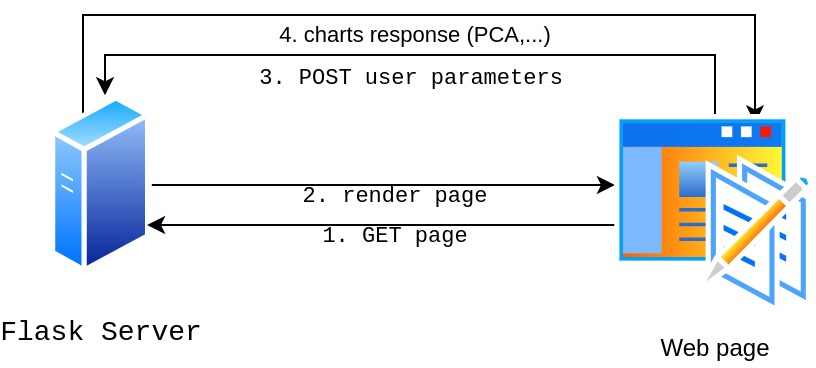
\includegraphics[scale=0.24,center]{./fig/ServerStructure.jpg}
	\label{fig:ss}
	\captionof{figure}{Summering schema to show the web app general structure.}
	
\end{figure}

\subsection{First page}
Due to the nature of the data, that involve countries from all around the world and time series data, we chose to start developing a map view. The first page is showed inside [Figure 2].

The cloropleth maps show how much the user selected countries have exported/imported to/from other ones in a user defined range of years between 1990-2018. The cloropleth map (from Greek $\chi\varpi\rho\sigma\varsigma$ "area/region" and $\phi\lambda\eta\theta\sigma\varsigma$ "multitude") is a kind of thematic map in which areas are shaded or patterned in proportion to a variable that represents an aggregate summary of a geographic features within each area, such as population density or per-capita income. We thought a cloropleth map could be usefult for our purpose and dataset. We implemented two of them (one for export and one for import) to ease the comparisons. In this case selecting a country, the other countries with which the selected country traded with, always in the same user defined range of years, are color shaded in proportion to the amount of units delivered  to them for the export map view, while received from them for the import view instead.

It was a critical part of our work in which we tried to find economic data to merge with our model, in order to relate economic value to traded weapons, and do more reasonable comparisons. The website of \textit{SIPRI} talks about an economic value associated to the transaction but we discovered in an advanced developing phase that it is not present in each entry. Despite the fact that the already mentioned \textit{TIV} value could have been useful for this purpose in this particular dataset \textit{SIPRI} did not included it at all. So with an expert in the field and some additional data, or with direct access to \textit{TIV} values, a linear combination could solve the problem in the future. However these considerations do not invalidate the main purpose of the analysis.

These maps along with a table showing the selected countries and some general information about them as \textit{GDP}, army dimension and population (as average for the selected range of years) compose the upper part of the page while at the bottom we can see a diverging bar chart showing at the same time the total number of exported weapons and imported ones for a determined year inside the user selected range. 

On its right we have the \textit{PCA} view, where computation of PCA is made using the already mentioned datasets. PCA is able to transform a selected number of features (min. three) dimensions space into a two dimensions space, letting explore cases in which we can identify the presence of clusters. Then continuing in this direction a barchart view shows the top fifteen most delivered weapon categories for the user selected range of years. Clicking one category text is possible to see a brief description about its characteristics but more details are contained in the second page that we will discuss later. Finally is always possible to look at filtered data inside the view containing the details about transactions.

%%% Big Figure
\begin{figure}[H]
	\centering
	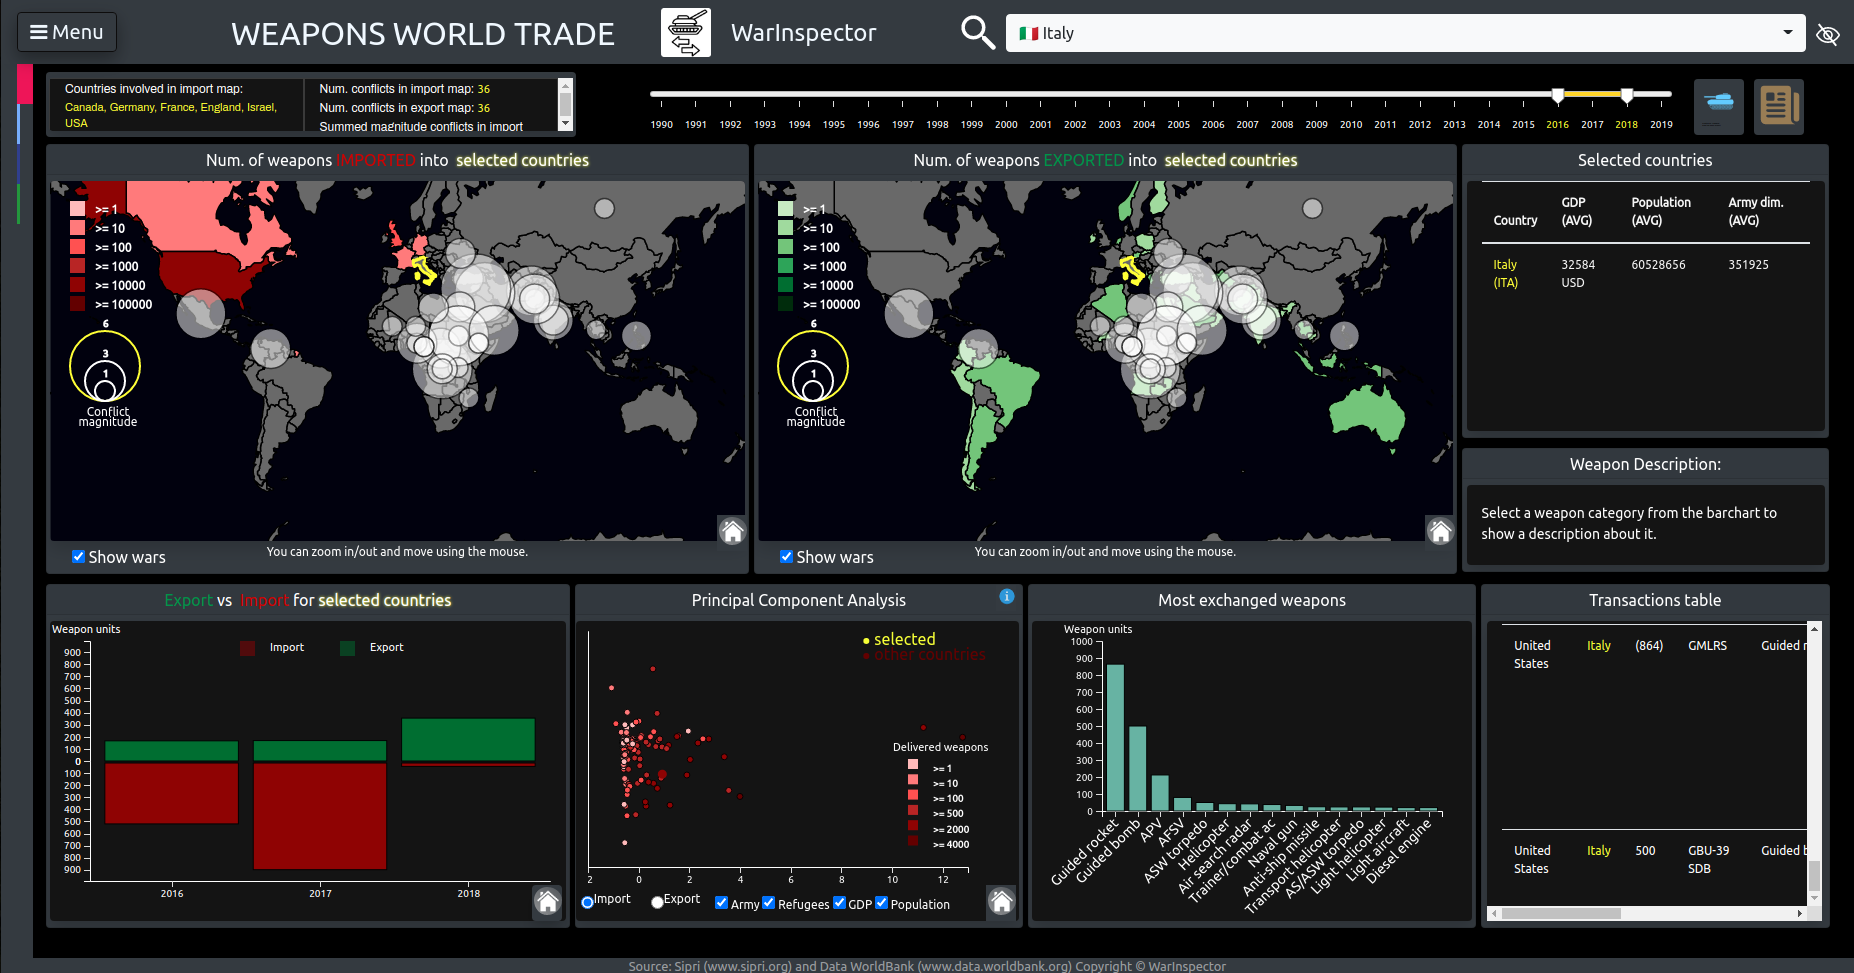
\includegraphics[scale=0.115,center]{./fig/screen1.png}
	\label{fig:va}
	\caption{System interface of the homepage of WarInspector.}
	
\end{figure}

\subsection{Second page}
In the second page [Figure 3] wanted the user to be able to explore the dataset analysing which are the most traded models and categories of weapons, with also a view on the possible trends of deliveries for a weapon model in specific ranges of years.
To do so we inserted three visualizations on the upper part of the page that show data analytics in a top-bottom fashion from left to right, where we start from macro categories of weapons and we move to single models. The first visualization is a barchart showing the most delivered weapon categories while on the right we emphasized the density of traded weapons for each year using  a heatmap. Interacting with the heatmap lets the user access the third visualization which is a connected scatterplot showing possible trends in the deliveries of a specific weapon through the years. 
This page is connected to the homepage by the presence of radio buttons that let the user switch from a global view of the trading of weapons to a dataset that is filtered according to the choices made on the homepage (years and countries of interest). 


\begin{figure}[H]
\centering
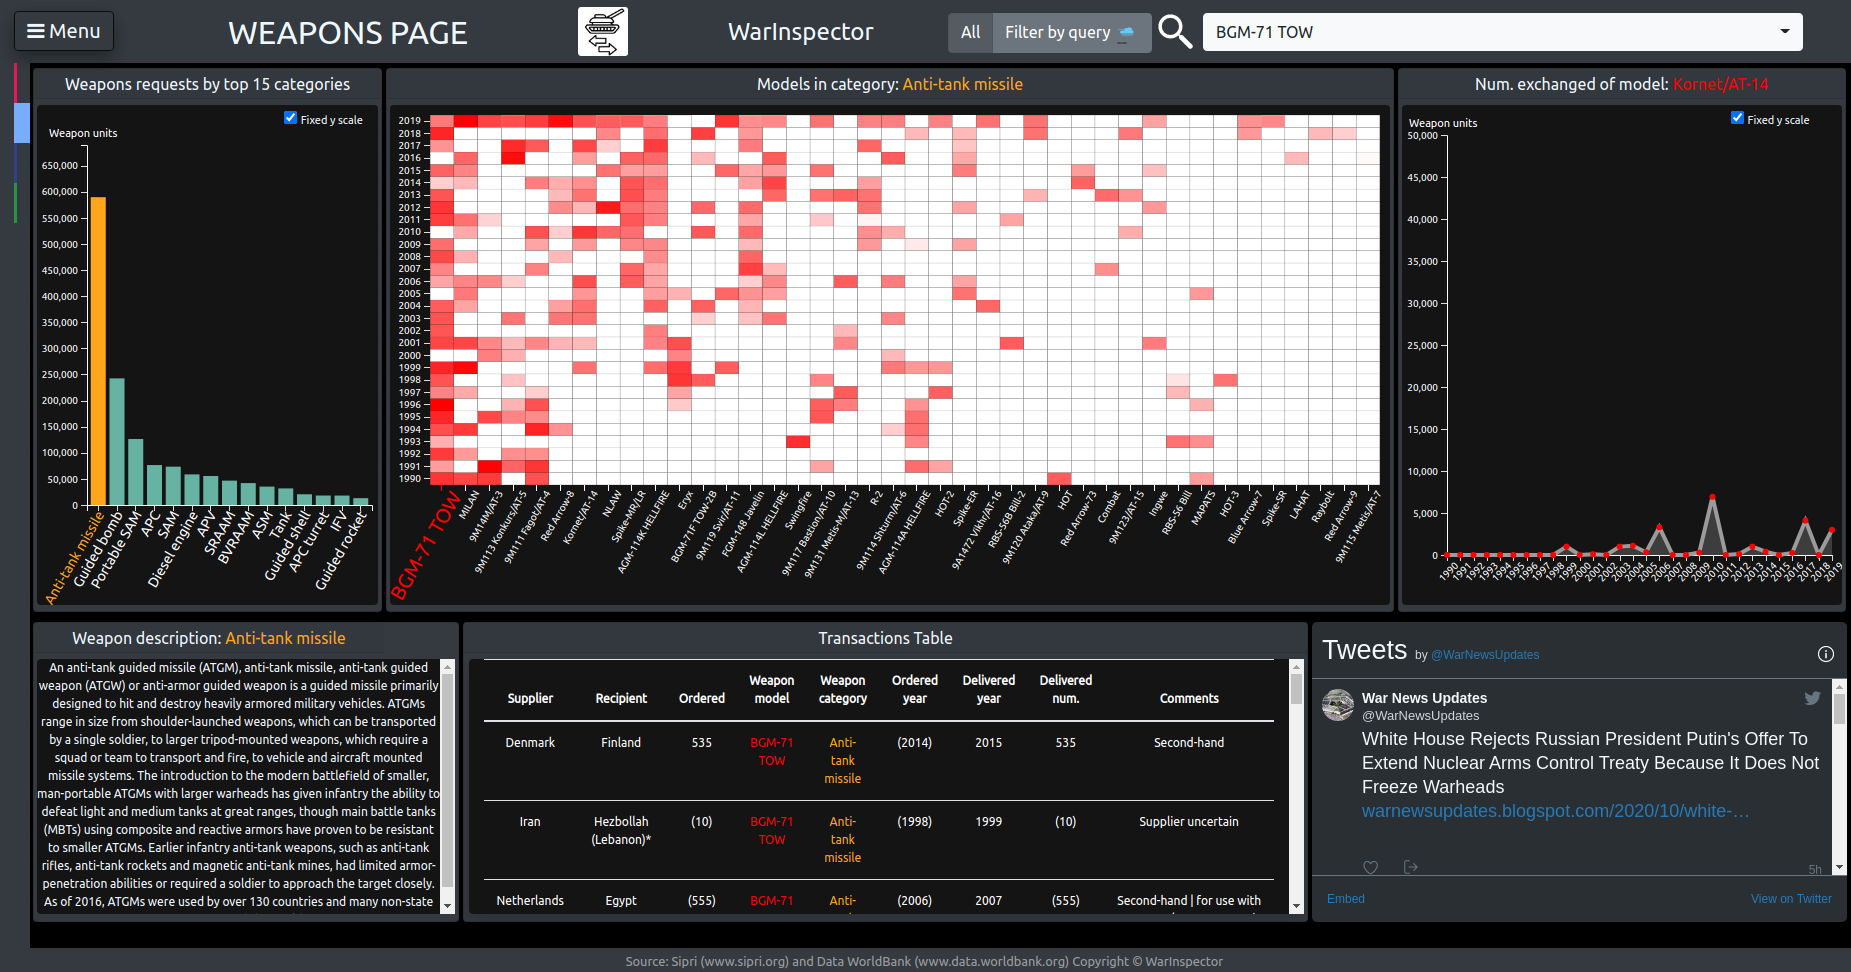
\includegraphics[scale=0.115,center]{./fig/screen2.png}
   \label{fig:va2}
    \caption{System interface of the weapons page of WarInspector.}

\end{figure}

\section{Visualization}
All the visualizations are contained inside card-like views, some of them like the maps and PCA enable zooming and panning and the possibility to reset to the start zoom and pan state.
Below we will discuss the main aspects of these visualizations.  
\subsection{Cloropleth map}
The two world maps use Mercator projection object to draw states and keep proportions when a zoom or a drag on the map is applied. Zoom and pan are coordinated among the two maps to ease the comparison between imports and exports. Countries have been drawn using \textit{topojson} mesh of a local file. Then at start and every time a slider/button changes the range of years and/or the supplier country of interest, a transition starts to fill the country with the correct color shade. In a second moment a bubble scatter was added to show conflicts happened through these years, where the radius of each circle represents the magnitude of the conflict.  

Import map countries are filled with different gradients of red  color proportional to the sum of the number of delivered units (computed using a group by and storing the result in a data structure) from the specified supplier to each state, always respecting the filtering. The range of colors, shown also in the legend visible to the user, is written below:
$$R_{tradedUnits}=\{1,10,100,1000,10000,100000\}$$

Several colors have been considered to be used, but green and red were chosen at the end, these two colors could express the economic nature of the transaction considering that exportations mean an economic entrance for the country (represented with green) while for importations is the opposite.
The drawbacks could be to give the user an implicit idea of “positive message” for green (whereas we are talking about war trading and in this case, possible military alliances, even with not democratic countries), while red could send the opposite message (whereas not every possible alliance should be considered dangerous, e.g. with border countries or in the same continent) and the problem of color blind subjects. To solve the last problem we introduced two diverging and color blindness safe colors, activated on button press, where the green turns into a lighter green color and the red into a pink color.


\subsection{Diverging bar chart}

The bar chart view was introduced to make possible a more clear comparison and it uses the same dataset of the other two views. Initially we introduced two distinct barcharts but later we gained some space on the page collapsing the two into one single diverging barchart where the upper bars show the user the total exports for a group of countries while the lower ones show the total imports. In this way the user can immediately see  if a certain year has more imports than export or viceversa, then looking at the maps and at the right barchart investigate the locations and weapons involved. The color tones are the same used in the maps (green for exports,...) without any color scale in this case but monotone colors instead.  

\subsection{PCA}
Using Principal component analysis we transform the coordinate space $X_s \subset R^n$ into a new one $Y_s \subset R^m$ where we know that this linear transformation preserves distances but can introduce false positives. The dimensions of sets is: $|R^n|=$ number of selected features, while $|R^m|=2$.
A deeper study about the best hyper-parameters could be done in this direction. 
Every point of the scatter plot is filled with a colour scale that express the total number of exported/imported delivered units.

\section{Interaction}
User can interact with all the views 
% (V1,V2 on \textit{Figure 1}) 
that are coordinated, acting both on the plots elements (bar for barplots and country surface for the maps,...) for the countries he wants to select and on the slider to choose the years between which the transactions happened.
%(I2 on \textit{Figure 1})
Also, a $<$select$>$ HTML element is present in both the pages on the top right corner of the page to select or deselect a country from a list showing the respective flag and name. Other possible interactions for the user are to act on both maps using the mouse, dragging (moving while click down) to move and zooming (using the mouse wheel) in or out. 

The top right corner is dedicated to buttons, here we have the
button guaranteeing the aforementioned possibility to switch the colors of the views to color blindness safe ones. Then we have a button to display the country considered at risks in the reference month and the button that redirects to the second page (focused on weapons) passing as parameters the features that can be used as filters.
For this purpose in the top middle portion of the screen in the second page, user has the possibility to filter or unfilter the dataset using the passed parameters through the use of radio buttons.

About the second page, the user can interact with the barplot and the heatmap. In the first case, changing category, the heatmap will be refreshed. In the second case, selecting a specific model, the plot will be refreshed. Beside them, the user can interact with other views, reading the description, the table with the greater transactions and finally Twitter banner, in order to have the last news about war topic.


\section{Discussion}

This section discusses the implications and limitations of our work and some design lessons we learned.
\subsection{Implications}
To the best of our knowledge, WarInspector is the first visual analytics interactive system that efficiently incorporates  global data of world arms trading. The availability of WarInspector together with some improvements and further SIPRI data could significantly promotes the exploration of global military trading in order to increase transparency in this field and possibly lead to historical conclusion that could move public opinion, revealing unsuspected influences of external countries in a conflict and maybe even predict some future events. 

\subsection{Limitations}

Some limitations are observed in our work. First, data found on SIPRI is considered highly accurate but it is naturally missing data from some countries (e.g. North Korea) that are unavailable for different reasons or distorted deliberately. Then PCA analysis uses rough distance measures that could show some patterns when big countries (e.g United States) stand out as expected but could not give enough room for deeper analysis.
As already mentioned in our work we sum up number of delivered units without considering the value of the units (e.g. hundreds of portable radio equipment is worth much less than one single fighter jet). This could lead easily, especially comparing low number exporter/importer, to false considerations. However it should be considered how just a simple economic analysis and report about the economic values of a weapon model or category could significantly improve the results.




\section{Conclusion}
Through the development of this project we learned more about the considerations and design choices that take place when working on a visual analytics project but also we faced the importance of a well formatted data to make comparisons and analysis easier and more reasonable.

\end{multicols}

\onecolumn{
\begin{thebibliography}{9}

\bibitem{d3} 
d3.js official page:
\\\texttt{https://d3js.org/}


\bibitem{latexcompanion} 
SIPRI datasets page:
\\\texttt{https://www.sipri.org/databases/armstransfers}

\bibitem{einstein} 
SIPRI page about sources and methods used:
\\\texttt{https://www.sipri.org/databases/milex/sources-and-methods}


\bibitem{worldData} 
Source for datasets external to SIPRI:
\\\texttt{https://data.worldbank.org/}


\bibitem{alertSource} 
Source for alert of countries currently at risk:
\\\texttt{https://www.crisisgroup.org/crisiswatch}

\bibitem{alertSource} 
Source for dataset of recent conflicts (we used some web scraping techniques):
\\\texttt{http://www.systemicpeace.org/warlist/warlist.htm}



\end{thebibliography}
}

\end{document}

